% style.tex -- shared preamble for the standalone test reports.
%
% Each report is an independent document: build it with
%   latexmk -xelatex -interaction=nonstopmode -halt-on-error -outdir=build <file>.tex
% from the reports/ directory. The main project report is intentionally not
% part of this directory; these reports document the test evidence on its own.

\documentclass[UTF8,a4paper,11pt]{ctexart}

\usepackage{geometry}
\geometry{top=2.3cm,bottom=2.3cm,left=2.5cm,right=2.5cm,headheight=14pt}

\usepackage{fontspec}
\setmainfont{DejaVu Serif}[AutoFakeSlant=0.2]
\setsansfont{DejaVu Sans}[AutoFakeSlant=0.2]
\setmonofont{DejaVu Sans Mono}[Scale=0.88]

\usepackage{amsmath,amssymb}
\usepackage{graphicx}
\graphicspath{{figures/}}
\usepackage{booktabs}
\usepackage{tabularx}
\usepackage{longtable}
\usepackage{array}
\usepackage{enumitem}
\usepackage{caption}
\usepackage{float}
\usepackage{xcolor}
\usepackage{listings}
\usepackage{fancyhdr}
\usepackage{hyperref}

\definecolor{codebg}{gray}{0.96}
\definecolor{codeframe}{gray}{0.45}
\lstset{
  basicstyle=\ttfamily\small,
  breaklines=true,
  breakatwhitespace=true,
  columns=fullflexible,
  keepspaces=true,
  frame=single,
  framerule=0.3pt,
  rulecolor=\color{codeframe},
  backgroundcolor=\color{codebg},
  showstringspaces=false,
  tabsize=2,
  aboveskip=0.7em,
  belowskip=0.7em,
}

% Inline code. detokenize preserves spaces and special characters; a plain
% lstinline argument loses spaces under ctex (xeCJK-listings turns them into
% CJK glue). Avoid a literal percent sign in the argument.
\newcommand{\code}[1]{\texttt{\detokenize{#1}}}

\pagestyle{fancy}
\fancyhf{}
\fancyhead[L]{\small 迷你搜索引擎项目}
\fancyhead[R]{\small 测试报告}
\fancyfoot[C]{\thepage}
\renewcommand{\headrulewidth}{0.4pt}
\fancypagestyle{plain}{%
  \fancyhf{}%
  \fancyfoot[C]{\thepage}%
  \renewcommand{\headrulewidth}{0pt}%
}

\captionsetup{font=small,labelfont=bf,skip=5pt}
\setlength{\parskip}{0.35em}
\setlength{\parindent}{2em}
\setlength{\emergencystretch}{3em}
\renewcommand{\arraystretch}{1.15}
\setlist{itemsep=0.2em,topsep=0.3em}

\hypersetup{
  colorlinks=true,
  linkcolor=blue!55!black,
  urlcolor=blue!55!black,
  bookmarksnumbered=true,
}

% Report title block: number/title, subtitle, version.
\newcommand{\reportheader}[3]{%
  \begin{center}
    {\large 迷你搜索引擎项目}\\[0.35em]
    {\LARGE\bfseries #1}\\[0.45em]
    {\large #2}\\[0.6em]
    {\small 版本 #3 \quad 测试日期 2026-10-19}
  \end{center}
  \vspace{0.3em}
  \noindent\rule{\linewidth}{0.6pt}
  \vspace{0.8em}
}

% A highlighted conclusion.
\newcommand{\finding}[1]{%
  \begin{quote}
    \noindent\textbf{结论：}#1
  \end{quote}
}


\begin{document}

\reportheader{测试报告 04：规模与 Bonus 测试}{SPIMI、v2 压缩、磁盘 B+Tree 与 500k 文件跑批}{1.0}
\hypersetup{pdftitle={测试报告 04：规模与 Bonus 测试}}

\begin{center}\small
\begin{tabularx}{0.92\linewidth}{@{}l X@{}}
  报告编号 & TR-04 \\
  被测对象 & \code{build-blocks}、\code{--compress}、B+Tree sidecar、500k 合成语料 \\
  被测版本 & 分支 \code{test/reports}，基于 \code{origin/main} 加注释与测试改动 \\
  测试环境 & WSL2（Linux 6.18），g++ 15.2，Release；合成语料 \\
  测试日期 & 2026-10-19 \\
  总体结论 & 500k 文件跑通；50M 键 B+Tree 实测；400M 词为外推而非实跑 \\
\end{tabularx}
\end{center}

\section{目标与范围}

课程 Bonus 问的是：如果拥有 500,000 个文件、400,000,000 个不同单词，程序还能不能工作。本报告测试三条可实测的扩展路径：

\begin{enumerate}
  \item \textbf{构建侧}：SPIMI 式块式外部构建，内存上界由块预算决定，而不是由总词表决定；
  \item \textbf{索引体积}：v2 差分 + varint 压缩；
  \item \textbf{查询侧}：磁盘 B+Tree 词典，term 不常驻内存。
\end{enumerate}

另外用 500,000 文件 / 20,000,000 token 的合成语料实际跑批，并把 B+Tree 实测到 50,000,000 键。\textbf{400M 词没有真正生成}（需要数百 GB 存储），报告明确区分实测与外推。

\section{测试环境与数据}

\begin{table}[H]
  \centering
  \caption{规模测试环境}
  \label{tab:scale-env}
  \small
  \begin{tabularx}{\linewidth}{@{}l X@{}}
    \toprule
    项目 & 值 \\
    \midrule
    系统 & WSL2，Linux 6.18，单机 \\
    编译器 & g++ 15.2，\code{-O2}，C++17 \\
    正式语料 & \code{data/}，195 文档，556,866 token（stopwords + stem） \\
    合成语料 & 500,000 文档 $\times$ 40 token，词表上限 5,000,000 \\
    正式索引 & v1 3,685,655 B；v2 1,725,694 B；sidecar 237,568 B \\
    \bottomrule
  \end{tabularx}
\end{table}

\section{构建侧：SPIMI 块式外部构建}

\code{mse build-blocks --block-terms N} 按文档流扫描，块内词典达到 $N$ 个 term 就排序落盘成 run，最后按词 $k$ 路归并。块边界只切在文档边界，因此同一词在后续 run 中的 docID 一定更大，归并时可以直接拼接 postings。

\subsection{正式语料}

\begin{table}[H]
  \centering
  \caption{SPIMI 块式构建（正式语料，budget 4096）}
  \label{tab:spimi-formal}
  \small
  \begin{tabularx}{0.72\linewidth}{@{}X r@{}}
    \toprule
    指标 & 数值 \\
    \midrule
    run 数 & 17 \\
    峰值活词 & 5,129（预算 + 单文档新增的合理超出） \\
    临时 run 字节 & 4,166,556 B \\
    扫描时间 & 0.36 s \\
    归并时间 & 0.06 s \\
    产物 & 与内存 \code{mse build} 逐字节一致 \\
    \bottomrule
  \end{tabularx}
\end{table}

\subsection{500k 文件合成语料}

\code{tools/gen_synthetic_corpus.py} 生成 500,000 个 plain 文档、每篇 40 token、词表上限 5,000,000。块式构建预算 50000：

\begin{table}[H]
  \centering
  \caption{500k 文件合成语料跑批}
  \label{tab:spimi-500k}
  \small
  \begin{tabularx}{0.85\linewidth}{@{}X r@{}}
    \toprule
    指标 & 数值 \\
    \midrule
    文档 / token & 500,000 / 20,000,000 \\
    不同词 & 4,908,747 \\
    run 数 / 峰值活词 & 398 / 50,039 \\
    临时 run 字节 & 558,397,200 B \\
    扫描 / 归并 & 9.98 s / 30.00 s \\
    峰值内存 & 1.50 GB \\
    索引 & 427,603,247 B \\
    内存构建对照 & 65.9 s / 2.43 GB，产物逐字节一致 \\
    \bottomrule
  \end{tabularx}
\end{table}

\finding{500k 文件侧已实际跑通；词表是 4.9M 而不是 400M。SPIMI 的峰值内存由块预算控制（实测 1.50 GB），不随 4.9M 词表线性增长。}

\section{索引体积：v2 差分 + 变长编码}

v2 把 postings 改为 docID gap、tf、position delta，每个整数使用字节对齐 varint；头部、文档表、term 表布局与 v1 相同，靠版本字段区分。

\begin{table}[H]
  \centering
  \caption{v2 压缩结果}
  \label{tab:v2}
  \small
  \begin{tabularx}{0.75\linewidth}{@{}l r r@{}}
    \toprule
    编码 & 索引字节 & 相对 v1 \\
    \midrule
    v1 原始 u32 & 3,685,655 & — \\
    v2 差分 + varint & \textbf{1,725,694} & \textbf{46.8\%} \\
    \bottomrule
  \end{tabularx}
\end{table}

正确性通过三条独立路径验证：

\begin{itemize}
  \item \code{brute_force.py} 独立解析 v2 文件，14,937 个词全项一致；
  \item \code{dump --verify-all} 对 v2 索引 + sidecar 校验 0 差异；
  \item varint 边界单元测试覆盖 6/14/22/30 位的上下界与截断拒绝。
\end{itemize}

\section{查询侧：磁盘 B+Tree 词典}

\code{mse build --dict-file} 把 term 到 (posting offset, length) 的映射冻结成页式 B+Tree sidecar。查询时只加载文档表，term 经 B+Tree 的 $O(\text{height})$ 页读定位，再 seek 到 posting 字节。

\begin{table}[H]
  \centering
  \caption{磁盘 B+Tree 词典（正式索引）}
  \label{tab:sidecar}
  \small
  \begin{tabularx}{0.85\linewidth}{@{}X r@{}}
    \toprule
    指标 & 数值 \\
    \midrule
    sidecar 大小 & 237,568 B（58 页 $\times$ 4 KiB，树高 2） \\
    占正式索引 & 6.4\% \\
    冷查询 \code{banquo} & 词典 2 页 + 索引 8,308 B $\approx$ 16.5 KB \\
    相对全量加载 & 0.45\% \\
    \code{--verify-all} & 14,937 词，0 mismatches \\
    页读 / 缓存命中 & 114 次页读，29,819 次缓存命中 \\
    查询输出 & 与全量加载文本/JSON 逐字节一致 \\
    \bottomrule
  \end{tabularx}
\end{table}

\section{B+Tree 规模实测}

\code{mse bptree-bench --keys N} 用递增 base-26 合成键 bulk-load 落盘，再用缓存 = 1 页的读取端做随机查询。

\begin{table}[H]
  \centering
  \caption{B+Tree 规模实测}
  \label{tab:bptree-scale}
  \small
  \begin{tabularx}{\linewidth}{@{}r r r r r r@{}}
    \toprule
    键数 & 树高 & 页数 & 文件大小 & 字节/键 & 每次查询页读 \\
    \midrule
    100,000 & 2 & 369 & 1,515,520 B & 15.16 & 2.00 \\
    1,000,000 & 3 & 3,688 & 15,110,144 B & 15.11 & 3.00 \\
    10,000,000 & 3 & 36,865 & 151,003,136 B & 15.10 & 3.00 \\
    30,000,000 & 3 & 110,593 & 452,993,024 B & 15.10 & 3.00 \\
    50,000,000 & 4 & 184,322 & 754,987,008 B & 15.10 & 4.00 \\
    \bottomrule
  \end{tabularx}
\end{table}

\begin{figure}[H]
  \centering
  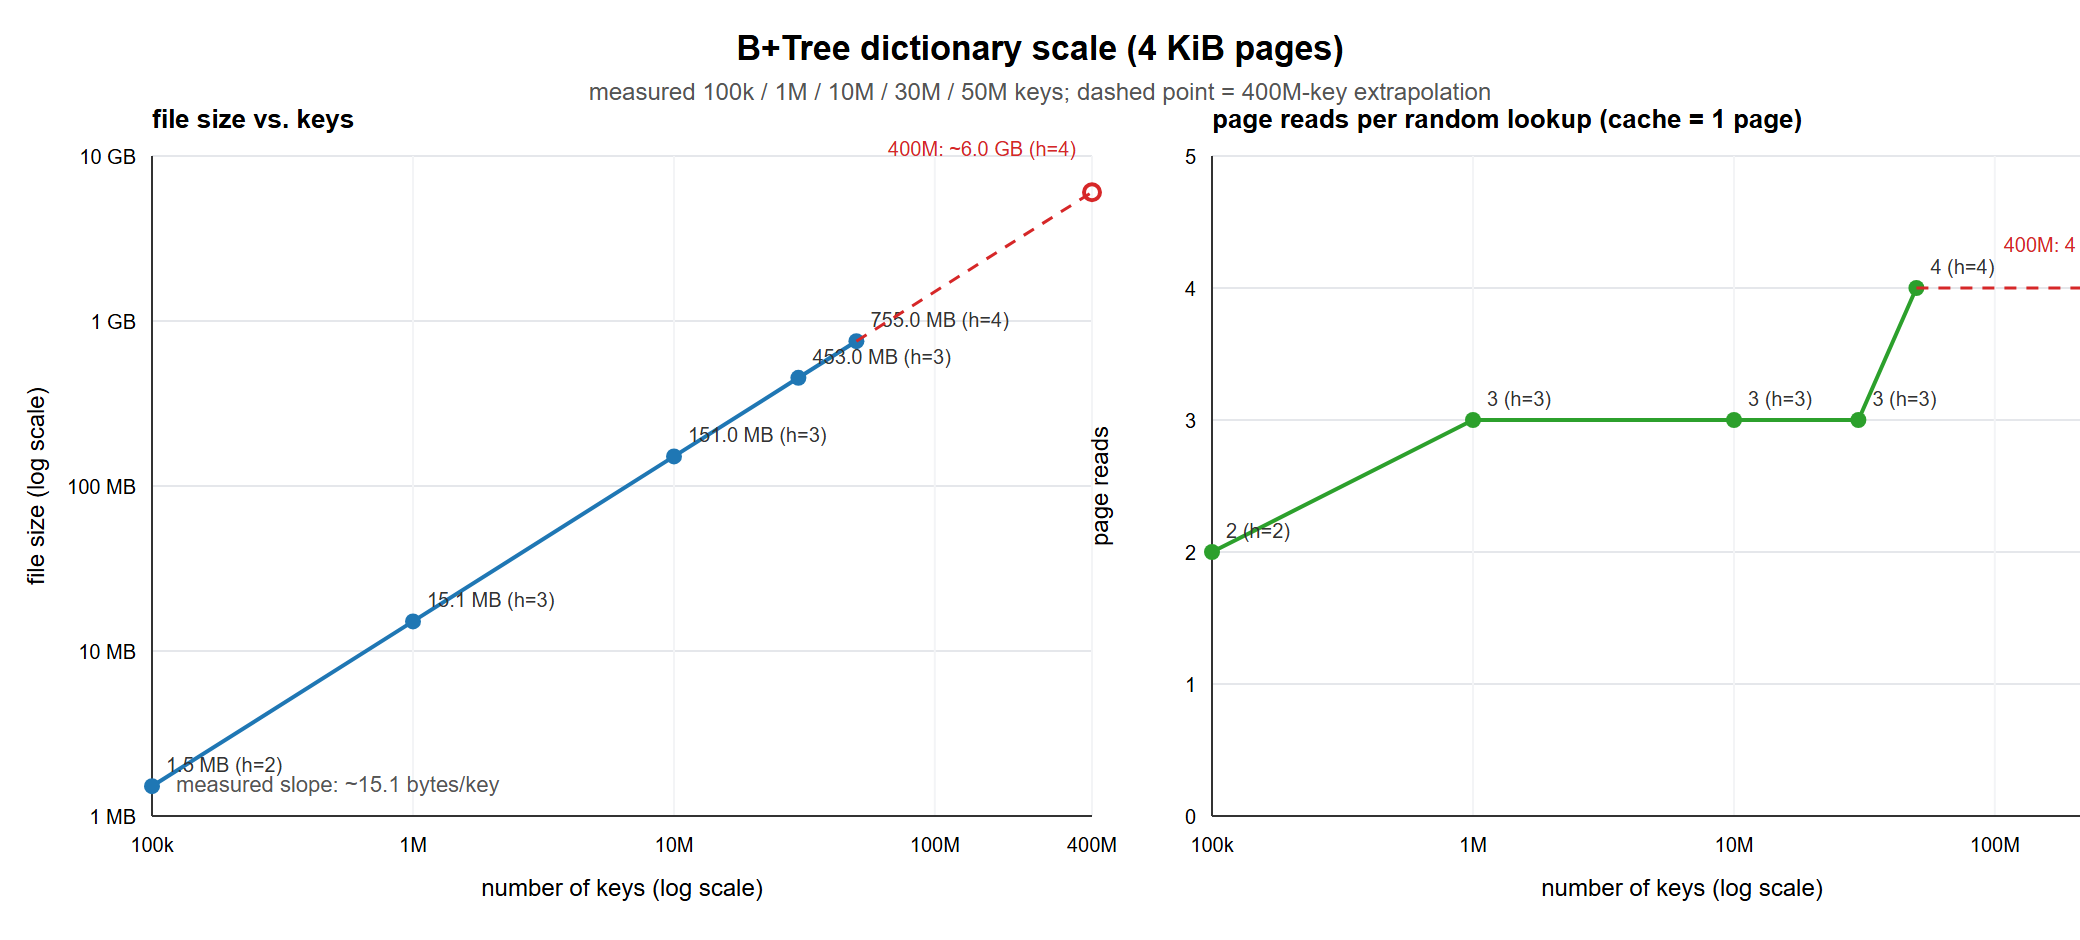
\includegraphics[width=0.95\linewidth]{figures/bptree_scale.png}
  \caption{B+Tree 规模实测。左图为文件大小（双对数），右图为每次随机查询的页读；400M 为按 15.1 B/键与扇出公式的外推点。}
  \label{fig:bptree-scale}
\end{figure}

体积严格线性（约 15.1 B/键），高度与扇出计算吻合。50M 键实测已进入 height 4、每次查询 4 页；按同一公式外推：

\begin{itemize}
  \item 100M 键 $\approx$ 1.5 GB，树高 4；
  \item 400M 键 $\approx$ 6.0 GB（取 6--6.5 GB），树高 4；
  \item 单次查询 4 页 $\approx$ 16 KB。
\end{itemize}

\section{第二语料：RFC}

\code{data2/} 收录 RFC 1035/5321/7231 三篇 plain 文本。用同一套 C++ 管线跑通：

\begin{table}[H]
  \centering
  \caption{RFC 第二语料端到端结果}
  \label{tab:rfc}
  \small
  \begin{tabularx}{\linewidth}{@{}l r@{}}
    \toprule
    指标 & 数值 \\
    \midrule
    文档 / 行 / token & 3 / 9,946 / 75,250 \\
    词型 & 4,328 \\
    动态熵停用词 & 58 词 \\
    索引词干 / posting / token & 2,660 / 4,594 / 45,370 \\
    索引大小 & 308,164 B \\
    brute-force 对拍 & 2,660 词全项一致 \\
    \code{count} CSV 对拍 & 与 Python 逐字节一致 \\
    \bottomrule
  \end{tabularx}
\end{table}

关键对照：RFC 2119 的 \code{must / may / should} 虽然 $df\_ratio=1.0$，但速率分布倾斜，未被熵规则误判为停用词。这说明“平”这个维度在跨语料场景真实起作用。

\section{边界与未完成项}

\begin{enumerate}
  \item \textbf{500k 文件已跑通，400M 词没有真正生成}：400M 个不同词需要数百 GB 存储，当前用 50M 键 B+Tree 实测 + 线性外推给出查询侧证据。
  \item \textbf{B+Tree 由内存索引 bulk-load}：查询侧已去掉常驻词典，构建侧仍需要先把索引放在内存；完整方案应让 SPIMI 归并直接产出 B+Tree 页文件。
  \item \textbf{32 位字段}：\code{posStart}/\code{tf} 在更大规模下应改 u64；\code{docID} 的 u32 对 500k 文件足够。
  \item \textbf{分布式未实现}：按文档切分与按词切分的权衡只有分析；GFS 式块复制/容错没有落地。
  \item \textbf{临时空间}：SPIMI 临时 run 约为语料的 2 倍；400M 词规模需要预算数百 GB 临时空间。
\end{enumerate}

\section{复现方式}

\begin{lstlisting}[language=bash]
# 正式语料 SPIMI
./build/mse build-blocks --stop-words data/stopwords.txt --stem \
    --block-terms 4096

# v2 压缩 + 磁盘 B+Tree
./build/mse build --index build/index-v2.bin \
    --stop-words data/stopwords.txt --stem --compress
./build/mse build --index build/index.bin --dict-file build/index.bpt \
    --stop-words data/stopwords.txt --stem
./build/mse dump --index build/index.bin --dict-file build/index.bpt --verify-all

# B+Tree 规模实测
./build/mse bptree-bench --keys 50000000 --lookups 1000

# 500k 合成语料（仅规模实验，不参与正式语料）
python3 tools/gen_synthetic_corpus.py --root build/scale-500k \
    --docs 500000 --tokens-per-doc 40 --vocab 5000000
./build/mse build-blocks --manifest build/scale-500k/data/manifest.tsv \
    --block-terms 50000 --index build/scale-500k-index.bin
\end{lstlisting}

\section{结论}

\begin{itemize}
  \item SPIMI 把构建内存从“词表规模”变成“块预算规模”：正式语料 17 个 run，500k 合成语料 398 个 run，峰值内存 1.50 GB；
  \item 500k 文件 / 20M token / 4.9M 词的构建已实际跑通，产物与内存构建逐字节一致；
  \item v2 把正式索引压到 v1 的 46.8\%，并通过独立解析与全词表校验；
  \item 磁盘 B+Tree 让查询只付树高次页读，正式索引冷查询约 16.5 KB（全量加载的 0.45\%）；
  \item 50M 键实测进入 height 4；400M 词约 6 GB、树高 4，为线性外推而非实跑；
  \item 距离完整 500k/400M 跑批还差工程集成与分布式，而不是算法上的未知。
\end{itemize}

\end{document}
